\documentclass[onlymath]{beamer}
% \documentclass[onlymath,handout]{beamer}

% Macros used by all lectures, but not necessarily by excercises

%%% General setup and dependencies:

% \usetheme[ddcfooter,nosectionnum]{tud}
\usetheme[nosectionnum,pagenum,noheader]{tud}
% \usetheme[nosectionnum,pagenum]{tud}

% Increase body font size to a sane level:
\let\origframetitle\frametitle
% \renewcommand{\frametitle}[1]{\origframetitle{#1}\normalsize}
\renewcommand{\frametitle}[1]{\origframetitle{#1}\fontsize{10pt}{13.2}\selectfont}
\setbeamerfont{itemize/enumerate subbody}{size=\small} % tud defaults to scriptsize!
\setbeamerfont{itemize/enumerate subsubbody}{size=\small}
% \setbeamerfont{normal text}{size=\small}
% \setbeamerfont{itemize body}{size=\small}

\renewcommand{\emph}[1]{\textbf{#1}}

\def\arraystretch{1.3}% Make tables even less cramped vertically

\usepackage[ngerman]{babel}
\usepackage[utf8]{inputenc}
\usepackage[T1]{fontenc}

%\usepackage{graphicx}
\usepackage[export]{adjustbox} % loads graphicx
\usepackage{import}
\usepackage{stmaryrd}
\usepackage[normalem]{ulem} % sout command
% \usepackage{times}
\usepackage{txfonts}
\usepackage{array}

% \usepackage[perpage]{footmisc} % reset footnote counter on each page -- fails with beamer (footnotes gone)
\usepackage{perpage}  % reset footnote counter on each page
\MakePerPage{footnote}

\usepackage{tikz}
\usetikzlibrary{arrows,positioning,decorations.pathreplacing}
% Inspired by http://www.texample.net/tikz/examples/hand-drawn-lines/
\usetikzlibrary{decorations.pathmorphing}
\pgfdeclaredecoration{penciline}{initial}{
    \state{initial}[width=+\pgfdecoratedinputsegmentremainingdistance,
    auto corner on length=1mm,]{
        \pgfpathcurveto%
        {% From
            \pgfqpoint{\pgfdecoratedinputsegmentremainingdistance}
                      {\pgfdecorationsegmentamplitude}
        }
        {%  Control 1
        \pgfmathrand
        \pgfpointadd{\pgfqpoint{\pgfdecoratedinputsegmentremainingdistance}{0pt}}
                    {\pgfqpoint{-\pgfdecorationsegmentaspect
                     \pgfdecoratedinputsegmentremainingdistance}%
                               {\pgfmathresult\pgfdecorationsegmentamplitude}
                    }
        }
        {%TO
        \pgfpointadd{\pgfpointdecoratedinputsegmentlast}{\pgfpoint{1pt}{1pt}}
        }
    }
    \state{final}{}
}
\tikzset{handdrawn/.style={decorate,decoration=penciline}}
\tikzset{every shadow/.style={fill=none,shadow xshift=0pt,shadow yshift=0pt}}
% \tikzset{module/.append style={top color=\col,bottom color=\col}}

% Use to make Tikz attributes with Beamer overlays
% http://tex.stackexchange.com/a/6155
\tikzset{onslide/.code args={<#1>#2}{%
  \only<#1| handout:0>{\pgfkeysalso{#2}}
}}
\tikzset{onslideprint/.code args={<#1>#2}{%
  \only<#1>{\pgfkeysalso{#2}}
}}

%%% Title -- always set this first

\newcommand{\defineTitle}[3]{
	\newcommand{\lectureindex}{#1}
	\title{Theoretische Informatik und Logik}
	\subtitle{\href{\lectureurl}{#1. Vorlesung: #2}}
	\author{\href{https://iccl.inf.tu-dresden.de/web/Markus_Kr\%C3\%B6tzsch}{Markus Kr\"{o}tzsch}\\[1ex]Lehrstuhl Wissensbasierte Systeme}
	\date{#3}
	\datecity{TU Dresden}
% 	\institute{CC-By 3.0, sofern keine anderslautenden Bildrechte angegeben sind}
}

%%% Table of contents:

\RequirePackage{ifthen}

\newcommand{\highlight}[2]{%
	\ifthenelse{\equal{#1}{\lectureindex}}{\alert{#2}}{#2}%
}

\def\myspace{-0.7ex}
\newcommand{\printtoc}{
\begin{tabular}{r@{$\quad$}l}
\highlight{1}{1.} & \highlight{1}{Willkommen/Einleitung formale Sprachen}\\[\myspace]
\highlight{2}{2.} & \highlight{2}{Grammatiken und die Chomsky-Hierarchie}\\[\myspace]
\highlight{3}{3.} & \highlight{3}{Endliche Automaten}\\[\myspace]
\highlight{4}{4.} & \highlight{4}{Complexity of FO query answering}\\[\myspace]
\highlight{5}{5.} & \highlight{5}{Conjunctive queries}\\[\myspace]
\highlight{6}{6.} & \highlight{6}{Tree-like conjunctive queries}\\[\myspace]
\highlight{7}{7.} & \highlight{7}{Query optimisation}\\[\myspace]
\highlight{8}{8.} & \highlight{8}{Conjunctive Query Optimisation / First-Order~Expressiveness}\\[\myspace]
\highlight{9}{9.} & \highlight{9}{First-Order~Expressiveness / Introduction to Datalog}\\[\myspace]
\highlight{10}{10.} & \highlight{10}{Expressive Power and Complexity of Datalog}\\[\myspace]
\highlight{11}{11.} & \highlight{11}{Optimisation and Evaluation of Datalog}\\[\myspace]
\highlight{12}{12.} & \highlight{12}{Evaluation of Datalog (2)}\\[\myspace]
\highlight{13}{13.} & \highlight{13}{Graph Databases and Path Queries}\\[\myspace]
\highlight{14}{14.} & \highlight{14}{Outlook: database theory in practice}
\end{tabular}
}

\newcommand{\overviewslide}{%
\begin{frame}\frametitle{Overview}
\printtoc
\medskip

Siehe \href{\lectureurl}{course homepage [$\Rightarrow$ link]} for more information and materials
\end{frame}
}

%%% Colours:
\usepackage{xcolor,colortbl}
\definecolor{redhighlights}{HTML}{FFAA66}
\definecolor{lightblue}{HTML}{55AAFF}
\definecolor{lightred}{HTML}{FF5522}
\definecolor{lightpurple}{HTML}{DD77BB}
\definecolor{lightgreen}{HTML}{55FF55}
\definecolor{darkred}{HTML}{CC4411}
\definecolor{darkblue}{HTML}{176FC0}%{1133AA}
\definecolor{nightblue}{HTML}{2010A0}%{1133AA}
\definecolor{alert}{HTML}{176FC0}
\definecolor{darkgreen}{HTML}{36AB14}
\definecolor{strongyellow}{HTML}{FFE219}
\definecolor{devilscss}{HTML}{666666}

\newcommand{\redalert}[1]{\textcolor{darkred}{#1}}

%%% Style commands

\newcommand{\quoted}[1]{\texttt{"}{#1}\texttt{"}}
\newcommand{\squote}{\texttt{"}} % straight quote
\newcommand{\Sterm}[1]{\ensuremath{\mathtt{\textcolor{purple}{#1}}}}    % letters in alphabets
\newcommand{\Snterm}[1]{\textsf{\textcolor{darkblue}{#1}}} % nonterminal symbols
\newcommand{\Sntermsub}[2]{\ensuremath{\Snterm{#1}_{\Snterm{#2}}}} % nonterminal symbols
\newcommand{\Slang}[1]{\textbf{\textcolor{black}{#1}}}    % languages
\newcommand{\Slangsub}[2]{\ensuremath{\Slang{#1}_{\Slang{#2}}}}    % languages
% Code
\newcommand{\Scode}[1]{\textbf{#1}}    % reserved words in program listings, e.g., "if"
\newcommand{\Scodelit}[1]{\textcolor{purple}{#1}}    % literals in program listings, e.g., strings
\newcommand{\Scomment}[1]{\textcolor{gray}{#1}}    % comment in program listings

\newcommand{\epstrastar}{\mathrel{\mathord{\stackrel{\epsilon}{\to}}{}^*}} % transitive reflexive closure of epsilon transitions in an epslion-NFA

\newcommand{\narrowcentering}[1]{\mbox{}\hfill#1\hfill\mbox{}}

\newcommand{\Smach}[1]{\ensuremath{\mathcal{#1}}}    % machines

\newcommand{\mytrue}{\Scodelit{1}}
\newcommand{\myfalse}{\Scodelit{0}}
% \newcommand{\emptyClause}{\bot}

\newcommand{\Scomplclass}[1]{{\textsc{#1}}} % font for complexity classes, used on slides where the "too many alphabets" LaTeX error appears when using the correct sc font :-(
% \newcommand{\complclass}[1]{\ensuremath{\mathsc{#1}}} % font for complexity classes

%%% Slide layout commands:

\newcommand{\sectionSlide}[1]{
\frame{\begin{center}
\LARGE
#1
\end{center}}
}
\newcommand{\sectionSlideNoHandout}[1]{
\frame<handout:0>{\begin{center}
\LARGE
#1
\end{center}}
}

\newcommand{\mydualbox}[3]{%
 \begin{minipage}[t]{#1}
 \begin{beamerboxesrounded}[upper=block title,lower=block body,shadow=true]%
    {\centering\usebeamerfont*{block title}#2}%
    \raggedright%
    \usebeamerfont{block body}
%     \small
    #3%
  \end{beamerboxesrounded}
  \end{minipage}
}
%
\newcommand{\myheaderbox}[2]{%
 \begin{minipage}[t]{#1}
 \begin{beamerboxesrounded}[upper=block title,lower=block title,shadow=true]%
    {\centering\usebeamerfont*{block title}\rule{0pt}{2.6ex} #2}%
  \end{beamerboxesrounded}
  \end{minipage}
}

\newcommand{\mycontentbox}[2]{%
 \begin{minipage}[t]{#1}%
 \begin{beamerboxesrounded}[upper=block body,lower=block body,shadow=true]%
    {\centering\usebeamerfont*{block body}\rule{0pt}{2.6ex}#2}%
  \end{beamerboxesrounded}
  \end{minipage}
}

\newcommand{\mylcontentbox}[2]{%
 \begin{minipage}[t]{#1}%
 \begin{beamerboxesrounded}[upper=block body,lower=block body,shadow=true]%
    {\flushleft\usebeamerfont*{block body}\rule{0pt}{2.6ex}#2}%
  \end{beamerboxesrounded}
  \end{minipage}
}

% label=180:{\rotatebox{90}{{\footnotesize\textcolor{darkgreen}{Beispiel}}}}
% \hspace{-8mm}\ghost{\raisebox{-7mm}{\rotatebox{90}{{\footnotesize\textcolor{darkgreen}{Beispiel}}}}}\hspace{8mm}
\newcommand{\examplebox}[1]{%
	\begin{tikzpicture}[decoration=penciline, decorate]
		\pgfmathsetseed{1235}
		\node (n1) [decorate,draw=darkgreen, fill=darkgreen!10,thick,align=left,text width=\linewidth, inner ysep=2mm, inner xsep=2mm] at (0,0) {#1};
% 		\node (n2) [align=left,text width=\linewidth,inner sep=0mm] at (n1.92) {{\footnotesize\raisebox{3mm}{\textcolor{darkgreen}{Beispiel}}}};
% 		\node (n2) [decorate,draw=darkgreen, fill=darkgreen!10,thick, align=left,text width=\linewidth,inner sep=2mm] at (n1.90) {{\footnotesize\raisebox{0mm}{\textcolor{darkgreen}{Beispiel}}}};
	\end{tikzpicture}%
}%

\newcommand{\codebox}[1]{%
	\begin{tikzpicture}[decoration=penciline, decorate]
		\pgfmathsetseed{1236}
		\node (n1) [decorate,draw=strongyellow, fill=strongyellow!10,thick,align=left,text width=\linewidth, inner ysep=2mm, inner xsep=2mm] at (0,0) {#1};
	\end{tikzpicture}%
}%

\newcommand{\defbox}[1]{%
	\begin{tikzpicture}[decoration=penciline, decorate]
		\pgfmathsetseed{1237}
		\node (n1) [decorate,draw=darkred, fill=darkred!10,thick,align=left,text width=\linewidth, inner ysep=2mm, inner xsep=2mm] at (0,0) {#1};
	\end{tikzpicture}%
}%

\newcommand{\theobox}[1]{%
	\begin{tikzpicture}[decoration=penciline, decorate]
		\pgfmathsetseed{1240}
		\node (n1) [decorate,draw=darkblue, fill=darkblue!10,thick,align=left,text width=\linewidth, inner ysep=2mm, inner xsep=2mm] at (0,0) {#1};
	\end{tikzpicture}%
}%

\newcommand{\anybox}[2]{%
	\begin{tikzpicture}[decoration=penciline, decorate]
		\pgfmathsetseed{1240}
		\node (n1) [decorate,draw=#1, fill=#1!10,thick,align=left,text width=\linewidth, inner ysep=2mm, inner xsep=2mm] at (0,0) {#2};
	\end{tikzpicture}%
}%


\newsavebox{\mybox}%
\newcommand{\doodlebox}[2]{%
\sbox{\mybox}{#2}%
	\begin{tikzpicture}[decoration=penciline, decorate]
		\pgfmathsetseed{1238}
		\node (n1) [decorate,draw=#1, fill=#1!10,thick,align=left,inner sep=1mm] at (0,0) {\usebox{\mybox}};
	\end{tikzpicture}%
}%

% Common notation

\usepackage{amsmath,amssymb,amsfonts}
\usepackage{xspace}

\newcommand{\lectureurl}{https://iccl.inf.tu-dresden.de/web/TheoLog2017}

\DeclareMathAlphabet{\mathsc}{OT1}{cmr}{m}{sc} % Let's have \mathsc since the slide style has no working \textsc

% Dual of "phantom": make a text that is visible but intangible
\newcommand{\ghost}[1]{\raisebox{0pt}[0pt][0pt]{\makebox[0pt][l]{#1}}}

\newcommand{\tuple}[1]{\langle{#1}\rangle}
\newcommand{\defeq}{\mathrel{:=}}

%%% Annotation %%%

\usepackage{color}
\newcommand{\todo}[1]{{\tiny\color{red}\textbf{TODO: #1}}}



%%% Old macros below; move when needed

\newcommand{\blank}{\text{\textvisiblespace}} % empty tape cell for TM

% table syntax
\newcommand{\dom}{\textbf{dom}}
\newcommand{\adom}{\textbf{adom}}
\newcommand{\dbconst}[1]{\texttt{"#1"}}
\newcommand{\pred}[1]{\textsf{#1}}
\newcommand{\foquery}[2]{#2[#1]}
\newcommand{\ground}[1]{\textsf{ground}(#1)}
% \newcommand{\foquery}[2]{\{#1\mid #2\}} %% Notation as used in Alice Book
% \newcommand{\foquery}[2]{\tuple{#1\mid #2}}

\newcommand{\quantor}{\mathord{\reflectbox{$\text{\sf{Q}}$}}} % the generic quantor

% logic syntax
\newcommand{\Inter}{\mathcal{I}} %used to denote an interpretation
\newcommand{\Jnter}{\mathcal{J}} %used to denote another interpretation
\newcommand{\Knter}{\mathcal{K}} %used to denote yet another interpretation
\newcommand{\Zuweisung}{\mathcal{Z}} %used to denote a variable assignment

% query languages
\newcommand{\qlang}[1]{{\sf #1}} % Font for query languages
\newcommand{\qmaps}[1]{\textbf{QM}({\sf #1})} % Set of query mappings for a query language

%%% Complexities %%%

\hyphenation{Exp-Time} % prevent "Ex-PTime" (see, e.g. Tobies'01, Glimm'07 ;-)
\hyphenation{NExp-Time} % better that than something else

% \newcommand{\complclass}[1]{{\sc #1}\xspace} % font for complexity classes
\newcommand{\complclass}[1]{\ensuremath{\mathsc{#1}}\xspace} % font for complexity classes

\newcommand{\ACzero}{\complclass{AC$_0$}}
\newcommand{\LogSpace}{\complclass{L}}
\newcommand{\NLogSpace}{\complclass{NL}}
\newcommand{\PTime}{\complclass{P}}
\newcommand{\NP}{\complclass{NP}}
\newcommand{\coNP}{\complclass{coNP}}
\newcommand{\PH}{\complclass{PH}}
\newcommand{\PSpace}{\complclass{PSpace}}
\newcommand{\NPSpace}{\complclass{NPSpace}}
\newcommand{\ExpTime}{\complclass{ExpTime}}
\newcommand{\NExpTime}{\complclass{NExpTime}}
\newcommand{\ExpSpace}{\complclass{ExpSpace}}
\newcommand{\TwoExpTime}{\complclass{2ExpTime}}
\newcommand{\NTwoExpTime}{\complclass{N2ExpTime}}
\newcommand{\ThreeExpTime}{\complclass{3ExpTime}}
\newcommand{\kExpTime}[1]{\complclass{#1ExpTime}}
\newcommand{\kExpSpace}[1]{\complclass{#1ExpSpace}}


\defineTitle{2}{Berechenbarkeit und Unentscheidbarkeit}{7. April 2017}

\begin{document}

\maketitle

\begin{frame}\frametitle{Was bisher geschah \ldots}\label{frame_hilbert}\label{frame_turing_child}

\begin{minipage}{2.3cm}
% ~\hspace{8mm}
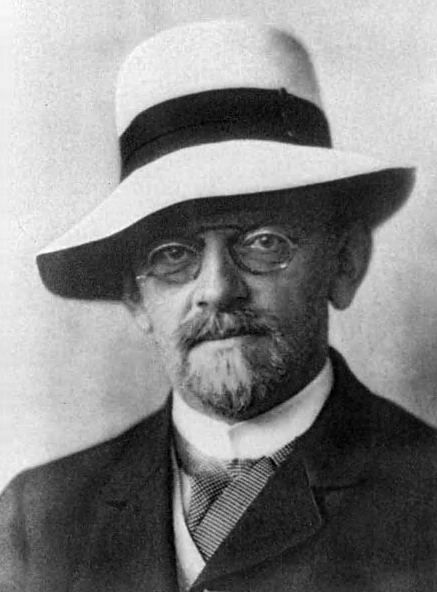
\includegraphics[width=2cm]{images/Hilbert}
\end{minipage}
\begin{minipage}{7.5cm}
Hilbert: "`Die Mathematik hat mehr als ein Problem. Wir brauchen ein formales Fundament! Dann kann jedes mathematische Problem durch endlich viele `Rechnenschritte' gelöst werden!"'
\end{minipage}

\bigskip

\begin{minipage}{7.3cm}
Turing: "`Es gibt Dinge, die man nicht berechnen kann. Ich kann das beweisen \ldots{} aber erst einmal muss ich definieren, was `berechnen' eigentlich bedeutet."'
\end{minipage}
\begin{minipage}{2.4cm}
~\hspace{4mm}
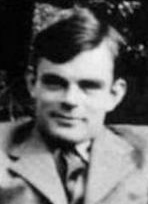
\includegraphics[width=2cm]{images/Turing}
\end{minipage}

\bigskip

Church und Turing (im Chor mit Kleene und Rosser):\\~\hfill"`Alle Computer sind gleich!"'\hfill~

\end{frame}

\begin{frame}\frametitle{Wichtige Typen von Turingmaschinen}

\begin{itemize}
\item \alert{Deterministische Turingmaschine} (DTM)
\item \alert{Nichtdeterministische Turingmaschine} (NTM)
\item \alert{Mehrband-Turingmaschine}\\
	Wir ändern die Definition so, dass statt einem Band in jedem Schritt $k\geq 2$ Bänder gelesen
	und beschrieben werden.\\
	Jedes Band hat einen unabhängigen Lese-/Schreibkopf.\\
	Die Eingabe wird auf das erste Band geschrieben.
\end{itemize}

\theobox{Satz: Deterministische und nichtdeterministische Turingmaschinen mit einer beliebigen Anzahl von Bändern können die gleichen Berechnungen ausführen.}

Details siehe Vorlesung Formale Systeme (Winter 2016/2017, Vorlesungen 18 und 19)

\end{frame}

\sectionSlide{Grundbegriffe: Berechnen und Entscheiden}

\begin{frame}\frametitle{TMs, die Mengen definieren}

Eine Turingmaschine kann eine Menge von akzeptierten Eingaben definieren:

\defbox{Die von einer TM $\Smach{M}$ \redalert{erkannte Sprache} $\Slang{L}(\Smach{M})$ ist die Menge aller Wörter, die von einer TM akzeptiert werden, d.h., bei deren Eingabe $\Smach{M}$
in einem Endzustand hält (DTM) / halten könnte (NTM).}\pause

Zwei Gründe für Nichtakzeptanz von Wörtern:
\begin{enumerate}[(1)]
\item TM hält in einem Zustand, der kein Endzustand ist
\item TM hält nicht (Endlosschleife)
\end{enumerate}
Es ist praktisch, wenn eine TM garantiert hält, da man Fall (2) meist nicht sicher erkennen kann (man weiß nicht, ob die TM irgendwann doch noch anhält)

\defbox{Eine TM ist ein \redalert{Entscheider}, wenn sie bei jeder Eingabe garantiert hält (bei NTMs: in jedem möglichen Lauf). Wir sagen in diesem Fall, dass die TM die von ihr erkannte Sprache \redalert{entscheidet}.}

\end{frame}

\begin{frame}\frametitle{TMs, die Funktionen definieren}

Eine Turingmaschine kann eine Funktion von Eingabewörtern auf Ausgabewörter definieren:

\defbox{Eine DTM $\Smach{M}$ \redalert{berechnet} eine partielle Funktion $f_{\Smach{M}}:\Sigma^*\to\Sigma^*$ wie folgt.
Für ein Wort $w\in\Sigma^*$ ist $f_{\Smach{M}}(w)=v$ wenn $\Smach{M}$ bei Eingabe $w$ mit einem Band anhält, auf dem 
nur $v$ steht, d.h., wenn der Bandinhalt nach dem Halten die Form $v\blank\blank\blank\cdots$ hat.}\pause

Es gibt also zwei Fälle, in denen $f_{\Smach{M}}(w)$ undefiniert ist:
\begin{enumerate}[(1)]
\item $\Smach{M}$ hält bei Eingabe $w$ mit einem Band, das nicht die geforderte Form hat
\item $\Smach{M}$ hält bei Eingabe $w$ gar nicht
\end{enumerate}

Das heißt: Wenn $f_{\Smach{M}}$ eine totale Funktion ist, dann muss $\Smach{M}$ immer halten.

\end{frame}

\begin{frame}\frametitle{Entscheidbarkeit und Berechenbarkeit}

Wir interessieren uns für Funktionen, die man berechnen kann:

\defbox{Eine totale oder partielle Funktion $f$ heißt \redalert{berechenbar}, wenn es eine DTM $\Smach{M}$ gibt, die $f$ berechnet, d.h. mit $f=f_{\Smach{M}}$.}

Anmerkung: Berechenbare totale Funktionen nennt man auch \redalert{rekursiv}; berechenbare partielle Funktionen \redalert{partiell rekursiv}.
\bigskip\pause

Bei Sprachen unterscheiden wir mehrere Fälle:

\defbox{Eine Sprache $\Slang{L}$ ist \redalert{entscheidbar} (=\redalert{berechenbar}=\redalert{rekursiv}), wenn es eine TM $\Smach{M}$ gibt,
die ihr Wortproblem entscheidet, d.h. $\Smach{M}$ ist Entscheider und $\Slang{L}=\Slang{L}(\Smach{M})$.
Andernfalls heißt $\Slang{L}$ \redalert{unentscheidbar}.\\[1ex]
%
$\Slang{L}$ ist \redalert{semi-entscheidbar} (=\redalert{Turing-erkennbar}=\redalert{Turing-akzeptierbar}=\redalert{rekursiv aufzählbar}) wenn
es eine TM $\Smach{M}$ gibt mit $\Slang{L}=\Slang{L}(\Smach{M})$, auch wenn $\Smach{M}$ kein Entscheider ist.}

\end{frame}

\begin{frame}\frametitle{Warum heißt es "`rekursiv aufzählbar"'?}

Bei rekursiv aufzählbaren Sprachen $\Slang{L}$ kann man eine TM konstruieren, die
alle Elemente von $\Slang{L}$ der Reihe nach "`aufzählt"':\bigskip

\defbox{Ein \redalert{Aufzähler} ist eine deterministische Turingmaschine $\Smach{M}$ mit einem speziellen
Zustand $q_{\textsf{Ausgabe}}$. Immer wenn $\Smach{M}$ in den Zustand $q_{\textsf{Ausgabe}}$
gelangt, wird der aktuelle Bandinhalt -- vom Anfang bis zum ersten Zeichen, nach dem nur noch $\blank$ folgen -- ausgegeben.\\[1ex]
%
Die \redalert{durch $\Smach{M}$ aufgezählte Sprache} ist die Menge aller Wörter
aus $\Sigma^*$, die $\Smach{M}$ ausgibt, wenn $\Smach{M}$ auf dem leeren Band gestartet wird.
}\bigskip

Die durch $\Smach{M}$ aufgezählte Sprache kann unendlich sein, wenn $\Smach{M}$ auf der leeren Eingabe nicht hält.
\bigskip

Es ist erlaubt, dass Wörter mehr als einmal in der Aufzählung vorkommen.

\end{frame}

\begin{frame}\frametitle{Beispiel für einen Aufzähler}

Wir betrachten das Alphabet $\Sigma=\{\Sterm{a},\Sterm{b}\}$

\begin{center}
\begin{tikzpicture}[baseline={(q1.base)}]
% \draw[help lines] (0,0) grid (7,2);
\node (q0) [circle,draw=black,thick] at (0,0) {$q_0$};
\node (q1) [circle,draw=black,thick] at (3,0) {$q_1$};
\node (q2) [rectangle,rounded corners=1.5ex, minimum height=2em,draw=black,thick] at (6,0) {$q_{\textsf{Ausgabe}}$};
%
\path[->,line width=0.5mm](-1,0) edge (q0);
\path[->,line width=0.5mm](q0) edge node[above] {$\blank\mapsto\Sterm{a},R$} (q1);
\path[->,line width=0.5mm](q1) edge node[above] {$\blank\mapsto\Sterm{b},N$} (q2);
\path[->,line width=0.5mm](q2) edge[bend left] node[below] {$\Sterm{b}\mapsto\Sterm{a},R$} (q0);
\end{tikzpicture}
\end{center}

\emph{Frage:} Welche Menge zählt diese TM auf?\pause\bigskip

\emph{Antwort:} $\{ \Sterm{a}^{2n+1}\Sterm{b}\mid 0\leq n\}$
\bigskip

Aufgabe zur Selbstkontrolle: Schreiben Sie einen Aufzähler für diese Sprache, ohne dabei die Bewegungsrichtung $N$ zu verwenden.

\end{frame}

\begin{frame}[t]\frametitle{Aufzählbar = semi-entscheidbar (1)}

\theobox{Satz: Eine Sprache $\Slang{L}$ ist genau dann semi-entscheidbar, wenn es
einen Aufzähler für $\Slang{L}$ gibt.
}\pause

\emph{Beweis:} "`$\Leftarrow$"' (Vom Aufzähler zur TM) Wenn es für $\Slang{L}$ einen Aufzähler
gibt, dann können wir $\Slang{L}$ wie folgt semi-entscheiden:
\begin{itemize}
\item Simuliere den Aufzähler auf einem leeren Band (wir dürfen eine Mehrband-TM verwenden).
\item Immer wenn $q_{\textsf{Ausgabe}}$ erreicht wird: vergleiche das Eingabeband mit dem Aufzählerband und akzeptiere, wenn beide das gleiche Wort beinhalten.
\item Andernfalls fahre mit der Aufzählung fort.
\item Falls die Aufzählung terminiert (ohne dass die Eingabe gefunden wurde), dann verwerfe.
\end{itemize}

\end{frame}

\begin{frame}[t]\frametitle{Aufzählbar = semi-entscheidbar (2)}

\theobox{Satz: Eine Sprache $\Slang{L}$ ist genau dann semi-entscheidbar, wenn es
einen Aufzähler für $\Slang{L}$ gibt.
}\pause

\emph{Beweis:} "`$\Rightarrow$"' (Von der TM zum Aufzähler) Wenn $\Slang{L}$ durch eine TM $\Smach{M}$ erkannt wird, dann können wir $\Slang{L}$ wie folgt aufzählen:
\begin{itemize}
\item Betrachte eine systematisch berechenbare Aufzählung aller Wörter $w_0, w_1, w_2, \ldots$ aus $\Sigma^*$
\item Für jede natürliche Zahl $n\geq 1$:
	\begin{itemize}
	\item Für jedes $i\in\{1,\ldots, n\}$:
		\begin{itemize}
		\item Simuliere $\Smach{M}$ auf Eingabe $w_i$ für $n$ Schritte
		\item Falls $\Smach{M}$ bei dieser Simulation terminiert und $w_i$ akzeptiert, dann gib $w_i$ aus
		\end{itemize}
	\end{itemize}
\end{itemize}
Anmerkung: Der so konstruierte Aufzähler terminiert nicht (selbst wenn die aufgezählte Menge endlich ist).\qed

\end{frame}

\begin{frame}\frametitle{Berechnungen jenseits von $\Sigma^*$}

\pause
Wir können den Berechnungsbegriff leicht auf beliebige Objekte ausdehnen, die als
Wörter kodiert werden können.
\bigskip

Wichtige Fälle:
\begin{itemize}
\item \alert{Natürliche Zahlen $\mathbb{N}$} können z.B. binär als Wörter über $\{\Sterm{0},\Sterm{1}\}$ kodiert werden
\item \alert{Tupel} (Listen) von Wörtern (oder natürlichen Zahlen, \ldots), können kodiert werden, indem man zum Eingabealphabet ein zusätzliches Trennzeichen $\#$ hinzufügt
\end{itemize}\bigskip\pause

\examplebox{Beispiel: Mithilfe dieser Kodierungen können wir z.B. von berechenbaren Funktionen $\mathbb{N}\to\mathbb{N}$ oder von
semi-entscheidbaren Teilmengen von $\mathbb{N}\times\mathbb{N}$ sprechen.}\medskip

Anmerkung: Oft gibt es viele denkbare Kodierungen eines Objektes als Wort. Vorerst sollen uns die Details nicht interessieren, solange klar ist, dass eine TM die Kodierung entschlüsseln kann.


\end{frame}


\begin{frame}\frametitle{Zusammenhang von Sprache und Funktion}

Berechenbarkeit von Funktionen und Sprachen sind eng verwandt.

\theobox{Eine Sprache $\Slang{L}$ ist genau dann entscheidbar, wenn die folgende Funktion $f:\Sigma^*\to\Sigma^*$ berechenbar ist (o.B.d.A. sei $\{\Sterm{0},\Sterm{1}\}\subseteq\Sigma$):
\[f(w)= \left\{\begin{array}{ll}
\Sterm{1} & \text{falls $w\in\Slang{L}$}\\
\Sterm{0} & \text{falls $w\notin\Slang{L}$}\\
\end{array}\right.\]}\pause

{\footnotesize
\emph{Beweisskizze:} "`$\Rightarrow$"' Ein Entscheider für $\Slang{L}$ kann in eine TM für $f$ umgebaut werden. Dazu verwendet man "`Subroutinen"', die den Bandinhalt löschen und mit einem einzelnen Zeichen \Sterm{1} oder \Sterm{0} ersetzten. Diese Routinen werden aufgerufen, wenn der ursprüngliche Entscheider halten würde: die \Sterm{1}-Routine beim Halten in einem Endzustand, die \Sterm{0}-Routine andernfalls.\medskip

{\tiny Eventuell muss man den Entscheider außerdem so modifizieren, dass das
Zeichen $\blank$ nur am Ende der verwendeten Bandinhaltes vorkommen kann (sonst wird das Löschen des gesamten Bandes problematisch!).

}
\smallskip

"`$\Leftarrow$"' Eine TM, die $f$ berechnet, kann in einen Entscheider für $\Slang{L}$ umgebaut werden. Die Idee ist wie zuvor, aber die Subroutinen prüfen jetzt, ob das Band \Sterm{1} oder \Sterm{0} enthält und wechseln entsprechend in einen akzeptierenden oder nicht-akzeptierenden Zustand.\qed

}

\end{frame}

\begin{frame}[t]\frametitle{Zusammenhang von Funktion und Sprache}

Für die Umkehrung stellen wir Funktionen als Mengen dar:

\theobox{Eine partielle Funktion $f$ ist genau dann berechenbar, wenn
$\textsf{Graph}_f=\{\tuple{w,f(w)}\mid w\in\Sigma^*,\; f(w)\text{ definiert}\}$ semi-entscheidbar ist.
Ist $f$ total, dann ist $\textsf{Graph}_f$ sogar entscheidbar.}

\pause
\emph{Beweis:} "`$\Rightarrow$"' Sei $f$ berechenbar. Dann kann man $\textsf{Graph}_f$ wie folgt
erkennen:
\begin{itemize}
\item Für eine Eingabe $\tuple{w,v}$, berechne $f(w)$ (als Subroutine).
\item Wenn die Berechnung von $f(w)$ terminiert, dann akzeptiere falls $f(w)=v$.
\item Wenn die Berechnung von $f(w)$ nicht terminiert, dann wird auch die Erkennung von $\textsf{Graph}_f$ nicht halten. Dieses Verhalten ist korrekt, da in diesem Fall $f(w)$ undefiniert ist und
$\tuple{w,v}\notin\textsf{Graph}_f$.
\end{itemize}\pause
Falls $f$ total ist, dann hält auch die Erkennung von $\textsf{Graph}_f$.

\end{frame}

\begin{frame}[t]\frametitle{Zusammenhang von Funktion und Sprache (2)}

Für die Umkehrung stellen wir Funktionen als Mengen dar:

\theobox{Eine partielle Funktion $f$ ist genau dann berechenbar, wenn
$\textsf{Graph}_f=\{\tuple{w,f(w)}\mid w\in\Sigma^*,\; f(w)\text{ definiert}\}$ semi-entscheidbar ist.
Ist $f$ total, dann ist $\textsf{Graph}_f$ sogar entscheidbar.}\pause

\emph{Beweis:} "`$\Leftarrow$"' Sei $\textsf{Graph}_f$ semi-entscheidbar. Dann kann
man $f$ wie folgt berechnen:
\begin{itemize}
\item Wir konstruieren einen Aufzähler für $\textsf{Graph}_f$ wie zuvor gezeigt
\item Der Aufzähler wird auf einem eigenen Band simuliert.
\item Immer wenn der Aufzähler ein Paar $\tuple{w,f(w)}$ ausgibt, vergleichen wir
	$w$ mit dem Inhalt des Eingabebandes
\item Wenn die Eingabe mit $w$ übereinstimmt, dann wird $f(w)$ als Ergebnis verwendet und die TM hält.
\item Andernfalls wird die Simulation der Aufzählung fortgesetzt.\qed
\end{itemize}

{\tiny
Anmerkung: Wir haben nicht formal definiert, was bei einer Mehrband-TM die Ausgabe ist, aber
das kann man leicht tun (oder die Mehrband-TM auf einem Band simulieren).

}
\end{frame}

\sectionSlide{Unentscheidbare Probleme}


\begin{frame}\frametitle{Es gibt unentscheidbare Probleme}

\theobox{Satz: Es gibt Sprachen und Funktionen, die nicht berechenbar sind.}

\pause
Dies kann man wie folgt zeigen:
\begin{itemize}
\item Die Menge der Turingmaschinen ist abzählbar
\item Die Menge der Sprachen über jedem Alphabet ist überabzählbar
\item Also muss es Sprachen geben, die durch keine TM entschieden werden.
\end{itemize}
\pause

Das Argument funktioniert analog mit (partiellen) Funktionen, deren Menge ebenfalls überabzählbar groß ist.\medskip

Das Argument zeigt zudem auch, dass die meisten Sprachen nicht einmal semi-entscheidbar sind (Kontrollfrage: Warum?).

\end{frame}

\begin{frame}\frametitle{Die Menge der TMs ist abzählbar}

\pause
Dies folgt in zwei Schritten:
\begin{itemize}
\item Jede TM kann leicht durch ein endliches Wort kodiert werden (z.B. binär)
\item Es gibt abzählbar viele Wörter. Man kann sie zum Beispiel wie folgt abzählen:
\begin{itemize}
\item Beginne mit dem leeren Wort $\epsilon$.
\item Reihe dann alle Wörter der Länge 1 auf
\item Reihe dann alle Wörter der Länge 2 auf
\item Reihe dann alle Wörter der Länge 3 auf
\item \ldots
\end{itemize}
\footnotesize
(Vgl. dazu auch Formale Systeme, Winter 2016/2017, Vorlesung 2)

\end{itemize}

\end{frame}

\begin{frame}\frametitle{Die Menge der Sprachen ist überabzählbar (1)}\label{frame_cantor}

\begin{minipage}{2.5cm}
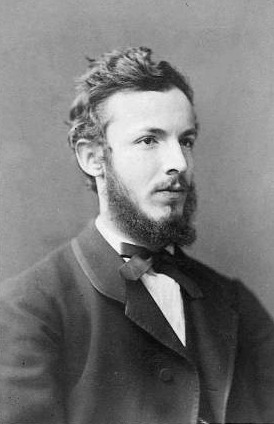
\includegraphics[width=2cm]{images/Cantor-1870}
\end{minipage}\pause%
\begin{minipage}{7.5cm}

Dies folgt aus einer Konstruktion von Georg Cantor:

\begin{itemize}
\item Beweis durch Widerspruch: Wir nehmen an, dass die Menge aller Sprachen abzählbar ist.
\item Sei $\Slangsub{L}{1},\Slangsub{L}{2},\Slangsub{L}{3}, \ldots$ eine entsprechende Aufzählung aller Sprachen.
\item Wir reihen außerdem alle Wörter in $\Sigma^*$ auf: $w_1, w_2, w_3, \ldots$.
\end{itemize}

\end{minipage}

\end{frame}

\begin{frame}\frametitle{Die Menge der Sprachen ist überabzählbar (2)}

\begin{itemize}
\item Man kann sich die Relation $\in$ zwischen Wörtern und Sprachen jetzt als unendliche Tabelle vorstellen:
%
\[ \begin{array}{l|c|c|c|c|c}
 & w_1 & w_2 & w_3 & w_4 & \ldots \\\hline
 \Slangsub{L}{1} & \only<2->{\cellcolor{purple!20}}\times & - & - & \times & \ldots \\\hline
 \Slangsub{L}{2} & - & \only<2->{\cellcolor{purple!20}}\times &  - & \times & \ldots \\\hline
 \Slangsub{L}{3} & - & \times & \only<2->{\cellcolor{purple!20}}- &  - & \ldots \\\hline
 \vdots & \vdots & \vdots & \vdots & \vdots & \ddots
 \visible<2->{\\\hline}
 \visible<2->{\Slangsub{L}{d} & - & - & \times & \ldots & }
\end{array}\]\pause
\item Wir konstruieren eine Sprache $\Slangsub{L}{d}$ durch \alert{Diagonalisierung}.\\
Formal: $w_i\in \Slangsub{L}{d}$ genau dann wenn $w_i\notin\Slangsub{L}{i}$.\pause
\end{itemize}
Dann kommt $\Slangsub{L}{d}$ in der Tabelle nicht vor. Widerspruch.

\end{frame}

\begin{frame}[t]\frametitle{Nichtwissen $\neq$ Unentscheidbarkeit}

Wie finden wir konkrete unentscheidbare Probleme?
\bigskip\pause

Es reicht nicht aus, dass wir nicht wissen, wie ein Problem algorithmisch gelöst werden kann!\bigskip

\examplebox{Beispiel: Sei $\Slang{L}_\pi$ die Menge aller endlichen Ziffernfolgen, die in der Dezimaldarstellung von $\pi$ vorkommen. Zum Beispiel gilt $\Sterm{14159265}\in\Slang{L}_\pi$ und $\Sterm{41}\in\Slang{L}_\pi$. \\[1ex]

\only<3->{%
Wir wissen nicht, ob man die Sprache $\Slang{L}_\pi$ entscheiden kann, aber sie könnte dennoch entscheidbar sein (z.B. wenn jede endliche Ziffernfolge irgendwo in $\pi$ vorkommt, was aber bisher nicht bekannt ist).}}

\end{frame}

\begin{frame}[t]\frametitle{Nichtwissen $\neq$ Unentscheidbarkeit (2)}

Es gibt sogar Fälle, in denen wir sicher sind, dass ein Problem entscheidbar ist,
aber trotztdem nicht wissen, wie man es löst.\\[1.5ex]\pause

\examplebox{Beispiel: Sei $\Slang{L}_{\pi7}$ die Menge aller Ziffernfolgen der Form $\Sterm{7}^n$, die in der Dezimaldarstellung von $\pi$ vorkommen.\\[1ex]

\only<3->{
$\Slang{L}_{\pi7}$ ist entscheidbar:
\begin{itemize}
\item Möglichkeit 1: $\pi$ enthält beliebig lange Ketten der Ziffer $\Sterm{7}$. Dann wird $\Slang{L}_{\pi7}$ durch eine TM entschieden, die alle Wörter der Form $\Sterm{7}^n$ akzeptiert.
\item Möglichkeit 2: $\pi$ enthält Ketten der Ziffer $\Sterm{7}$ nur bis zu einer maximalen Länge $\ell$. Dann wird $\Slang{L}_{\pi7}$ durch eine TM entschieden, die alle Wörter der Form $\Sterm{7}^n$ mit $n\leq\ell$ akzeptiert.
\end{itemize}
Für jeden denkbaren Fall gibt es einen Algorithmus -- wir wissen nur nicht, welcher davon korrekt ist.}
}

\end{frame}

\newcommand{\bbfunc}{\boldsymbol{\Sigma}}

\begin{frame}[t]\frametitle{Ein erstes unentscheidbares Problem (1)}

\emph{Frage:} Falls eine TM anhält, wie lange kann das im schlimmsten Fall dauern?\\
\bigskip\pause

\emph{Antwort:} Beliebig lange, weil:
\begin{enumerate}[(a)]
\item die Eingabe beliebig groß sein kann
\item die TM beliebig groß sein kann
\end{enumerate}

\end{frame}

\begin{frame}[t]\frametitle{Ein erstes unentscheidbares Problem (2)}

\emph{Frage:} Falls eine TM \alert{mit $n$ Zuständen} und \alert{einem zwei-elementigem Arbeitsalphabet $\Gamma=\{\Sterm{x}, \blank\}$} auf einem \alert{leeren Band} anhält, wie lange kann das im schlimmsten Fall dauern?\\
\bigskip\pause

\emph{Antwort:} Das kommt auf $n$ an \ldots\bigskip\pause

\defbox{Wir definieren $S(n)$ als die maximale Zahl an Schritten ist, die eine DTM mit
$n$ Zuständen und dem Arbeitsalphabet $\Gamma=\{\Sterm{x}, \blank\}$ auf dem leeren Band ausführt, bevor sie schließlich hält.}

\emph{Beobachtung:} $S$ ist wohldefiniert.
\begin{itemize}
\item Die Zahl der TMs mit maximal $n$ Zuständen ist endlich
\item Unter den relevanten $n$-Zustand-TMs, gibt es eine maximale Anzahl an Schritten bis zum Halten (TMs die nicht halten werden ignoriert)
\end{itemize}

\end{frame}

\begin{frame}\frametitle{Fleißige Biber}\label{frame_rado}

\begin{minipage}[b]{7.5cm}
Eine leichte Abwandlung des Schrittzählers ist\\das Busy-Beaver-Problem:
\end{minipage}%
\begin{minipage}[t]{2.5cm}
~\hspace{2mm}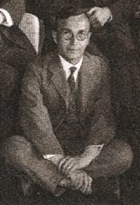
\includegraphics[width=2cm]{images/Rado}\\
{\tiny \mbox{}\hspace{2mm}Tibor Rad\'{o}, BB-Erfinder}
\end{minipage}\bigskip


\defbox{Die \redalert{Busy-Beaver-Funktion} $\bbfunc:\mathbb{N}\to\mathbb{N}$ ist eine totale Funktion, wobei $\bbfunc(n)$ die maximale Zahl an $\Sterm{x}$ ist, die eine DTM mit höchstens
$n$ Zuständen und dem Arbeitsalphabet $\Gamma=\{\Sterm{x}, \blank\}$ beginnend mit dem leeren Band schreiben kann, bevor sie schließlich hält.}

Anmerkung: Der genaue Wert von $\bbfunc(n)$ hängt von Details der TM-Definition ab.\\[0.5ex]
{\footnotesize Üblich ist hier insbesondere die Verwendung eines zweiseitig unendlichen Bands, das man bei Bedarf nach links und rechts erweitern kann.

}

\end{frame}

\begin{frame}\frametitle{Beispiel}

Die Busy-Beaver-Zahl $\bbfunc(2)$ ist $4$, wenn man ein beidseitig unendliches Band annimmt.\\
Die folgende TM realisiert dieses Verhalten:

\begin{center}
\begin{tikzpicture}[baseline={(q1.base)}]
% \draw[help lines] (0,0) grid (7,2);
\node (A) [circle,draw=black,thick] at (0,0) {$A$};
\node (B) [circle,draw=black,thick] at (3,0) {$B$};
%
\path[->,line width=0.5mm](-1,0) edge (A);
\path[->,line width=0.5mm](A) edge[bend left] node[above,align=left] {$\blank\mapsto\Sterm{x},R$\\$\Sterm{x}\mapsto\Sterm{x},L$} (B);
\path[->,line width=0.5mm](B) edge[bend left] node[below] {$\blank\mapsto\Sterm{x},L$} (A);
\end{tikzpicture}
\end{center}

Wir erhalten: $A\blank\vdash \Sterm{x}B\blank\vdash A\Sterm{xx}\vdash B\blank\Sterm{xx}\vdash A\blank\Sterm{xxx}\vdash \Sterm{x}B\Sterm{xxx}$

\end{frame}

\begin{frame}\frametitle{Busy-Beaver berechnen?}

% Wie schwer kann das schon sein \ldots?\pause

\theobox{Satz: Die Busy-Beaver-Funktion ist nicht berechenbar.}

\pause
\emph{Beweisskizze:} Nehmen wir an, $\bbfunc$ wäre berechenbar.\pause
\begin{itemize}
\item Dann kann man eine TM $\Smach{M}_{\bbfunc}$ erzeugen, die mit dem Alphabet $\{\Sterm{x},\blank\}$ arbeitet und die Funktion $\Sterm{x}^n\mapsto\Sterm{x}^{f(n)}$ berechnet.\pause
\item Sei $\Smach{M}_{+1}$ eine TM, welche die Funktion $\Sterm{x}^n\mapsto\Sterm{x}^{n+1}$ berechnet.\pause
\item Sei $\Smach{M}_{\times2}$ eine TM, welche die Funktion $\Sterm{x}^n\mapsto\Sterm{x}^{2n}$ berechnet.\pause
\item Sei $k$ die Gesamtzahl der Zustände in $\Smach{M}_{\bbfunc}$, $\Smach{M}_{+1}$ und $\Smach{M}_{\times2}$. Es gibt eine TM $\Smach{I}_k$ mit $k$ Zuständen, die das Wort $\Sterm{x}^k$ auf das leere Band schreibt.\pause
\item Wenn man nun hintereinander $\Smach{I}_k$, $\Smach{M}_{\times2}$, $\Smach{M}_{\bbfunc}$ und $\Smach{M}_{+1}$ ausführt, dann erhält man eine TM mit $2k$ Zuständen, die insgesamt $\bbfunc(2k)+1$ mal $\Sterm{x}$ schreibt und dann hält.\pause
\item Also ist $\bbfunc(2k)\geq\bbfunc(2k)+1$ -- Widerspruch.\qed
\end{itemize}


\end{frame}

\begin{frame}\frametitle{Bemerkungen zum Beweis}

\emph{Anmerkung 1:} Der Beweis verwendet die interessante Idee, dass man TMs als "`Subroutinen"' von anderen TMs verwenden kann. Wir werden das noch mehr verwenden.
\bigskip

\emph{Anmerkung 2:} Der Schritt von einer beliebigen Berechnung einer Funktion $f:\mathbb{N}\to\mathbb{N}$ zu einer TM, die eine Funktion $\Sterm{x}^n\mapsto \Sterm{x}^{f(n)}$ berechnet, ist nicht schwer; man ändert nur die Kodierung der Ein- und Ausgabe von binär auf unär.
\bigskip

\emph{Anmerkung 3:} Der Schritt von einer beliebigen TM zu einer, die auf dem Alphabet $\{\Sterm{x},\blank\}$ arbeitet, ist etwas kniffliger, aber machbar.

\end{frame}

\begin{frame}\frametitle{Theorie und Praxis}

\textcolor{darkred}{
"`Unentscheidbarkeit ist doch eine rein theoretische Eigenschaft! In der Praxis ist es egal, ob wir $\bbfunc(n)$ für beliebig große $n$ berechnen können. Die praktisch relevanten Fälle können wir sicher klären."'}
\bigskip\pause

Nun ja \ldots{} seit den 1960ern ist man noch nicht so weit gekommen:\medskip

\begin{tabular}{@{}rllllllll@{}}
$n$:          & $1$ & $2$ & \visible<3->{$3$} & \visible<4->{$4$}  & \visible<5->{$5$} & \visible<6->{$6$} & \visible<7->{$7$} & \visible<8->{$8$} \\\hline
$\bbfunc(n)$: & $1$ & $4$ & \visible<3->{$6$} & \visible<4->{$13$} & \visible<5->{$\geq 4098$} & \visible<6->{$\geq 3,5\times 10^{18267}$} & \visible<7->{riesig} & \visible<8->{irrsinnig}
\end{tabular}
\bigskip

\visible<9->{
Für $n=10$ kann man eine untere Schranke der Form $\bbfunc(10)>3^{3^{3^{.^{.^{.^3}}}}}$ angeben, wobei der komplette Ausdruck über $7,6$ Billionen mal die Zahl $3$ enthält.}

\end{frame}


\begin{frame}\frametitle{Zusammenfassung und Ausblick}

Turingmaschinen sind auf viele Arten verwendbar (und definierbar)
\bigskip

Funktionen und Mengen können berechenbar sein, aber die meisten sind es nicht
\bigskip

Semi-entscheidbare Mengen können durch Aufzähler erzeugt werden
\bigskip

Die Busy-Beaver-Funktion ist nicht berechenbar und wächst irrsinnig schnell
\bigskip

\anybox{yellow}{
Was erwartet uns als nächstes?
\begin{itemize}
\item Relevantere Probleme
\item Reduktionen
\item Rechenmodelle, die nicht auf TMs beruhen
\end{itemize}
}

\end{frame}

\begin{frame}[t]\frametitle{Bildrechte}

Folie \ref{frame_hilbert}: gemeinfrei\\
Folie \ref{frame_cantor}: Fotografie von 1870, gemeinfrei\\
Folie \ref{frame_rado}: Ausschnitt aus einer Fotografie von 1928, \url{http://www.bibl.u-szeged.hu/sztegy/photo/778.jpg}, CC-By-SA 3.0\\

\end{frame}


\end{document}